\subsection*{Library Description}
\begin{frame}[t]
  %\frametitle{LibMesh Tree}
%  \vspace{-.25in}
%  \begin{center}
%    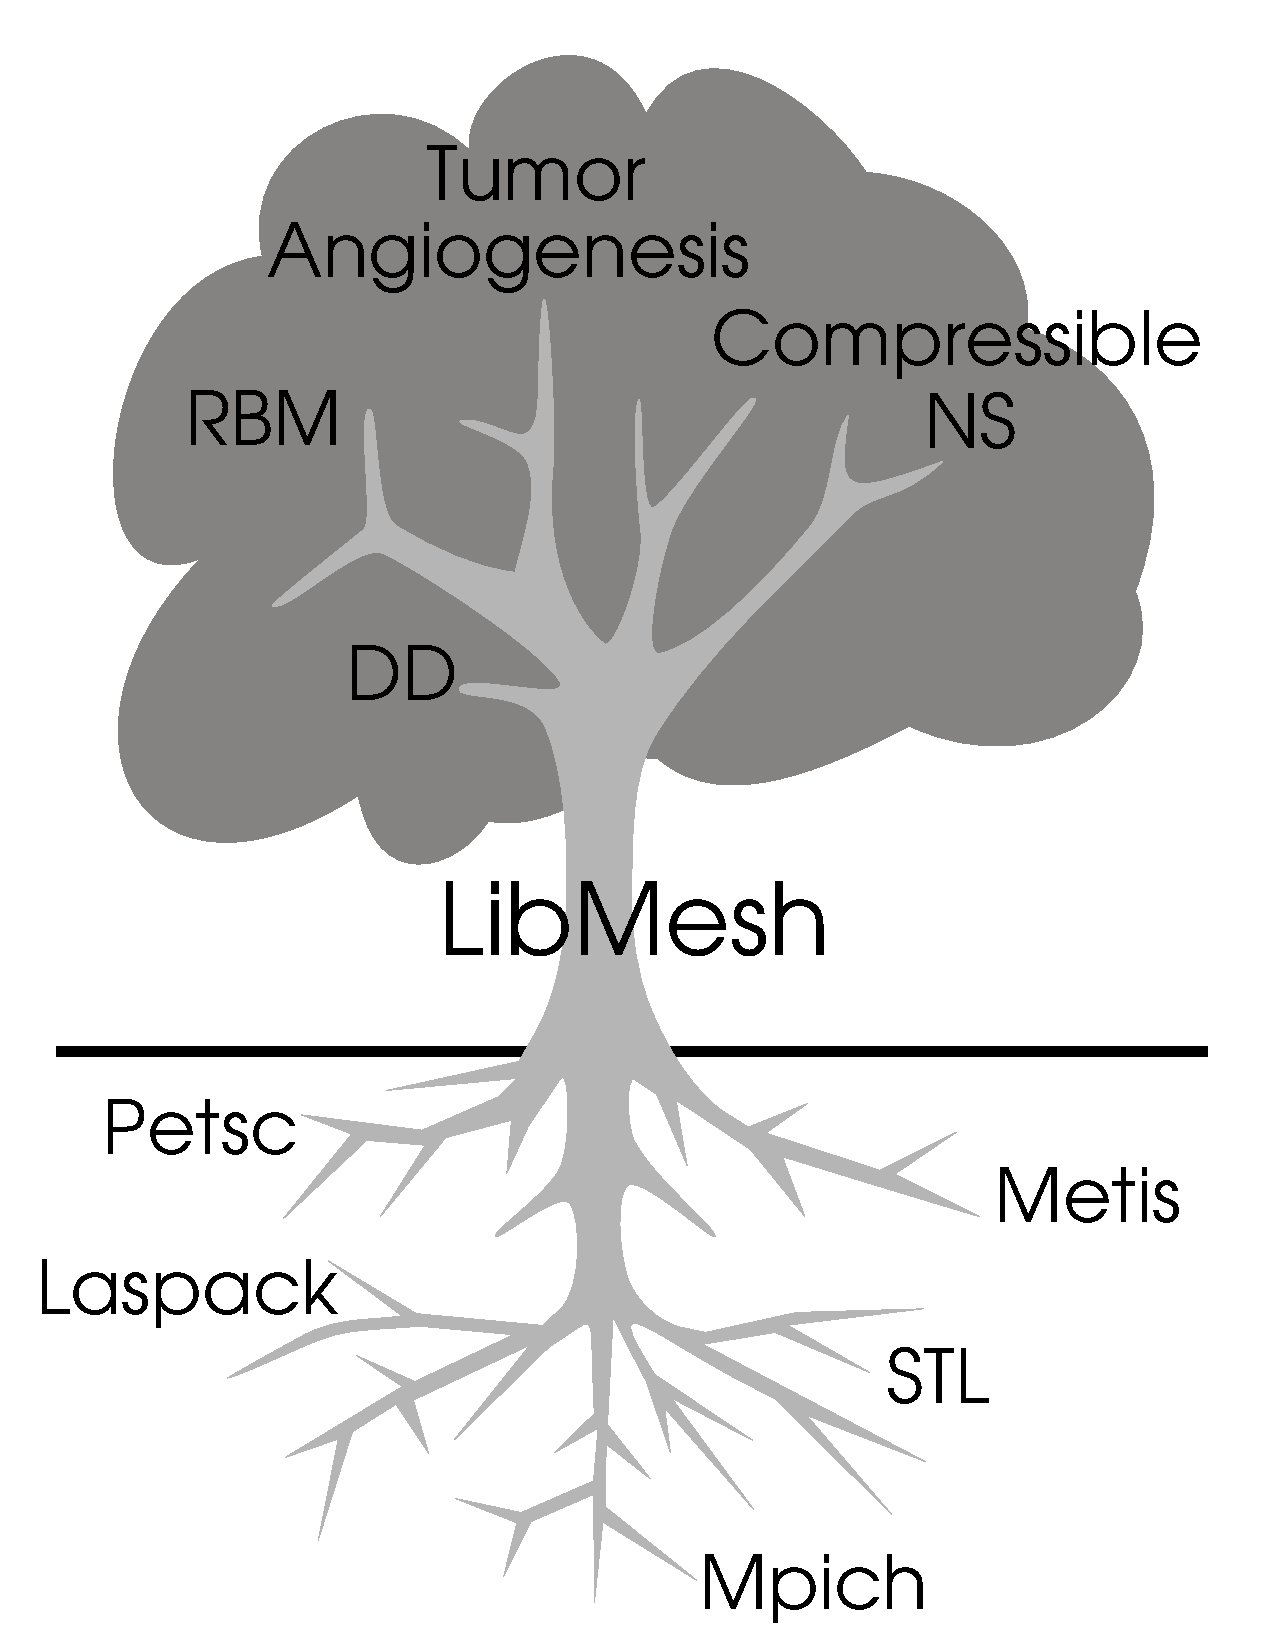
\includegraphics[width=.6\textwidth]{mytreeandroots_allnames}    
%  \end{center}


    \begin{minipage}[h]{.6\textwidth}
    \begin{center}
      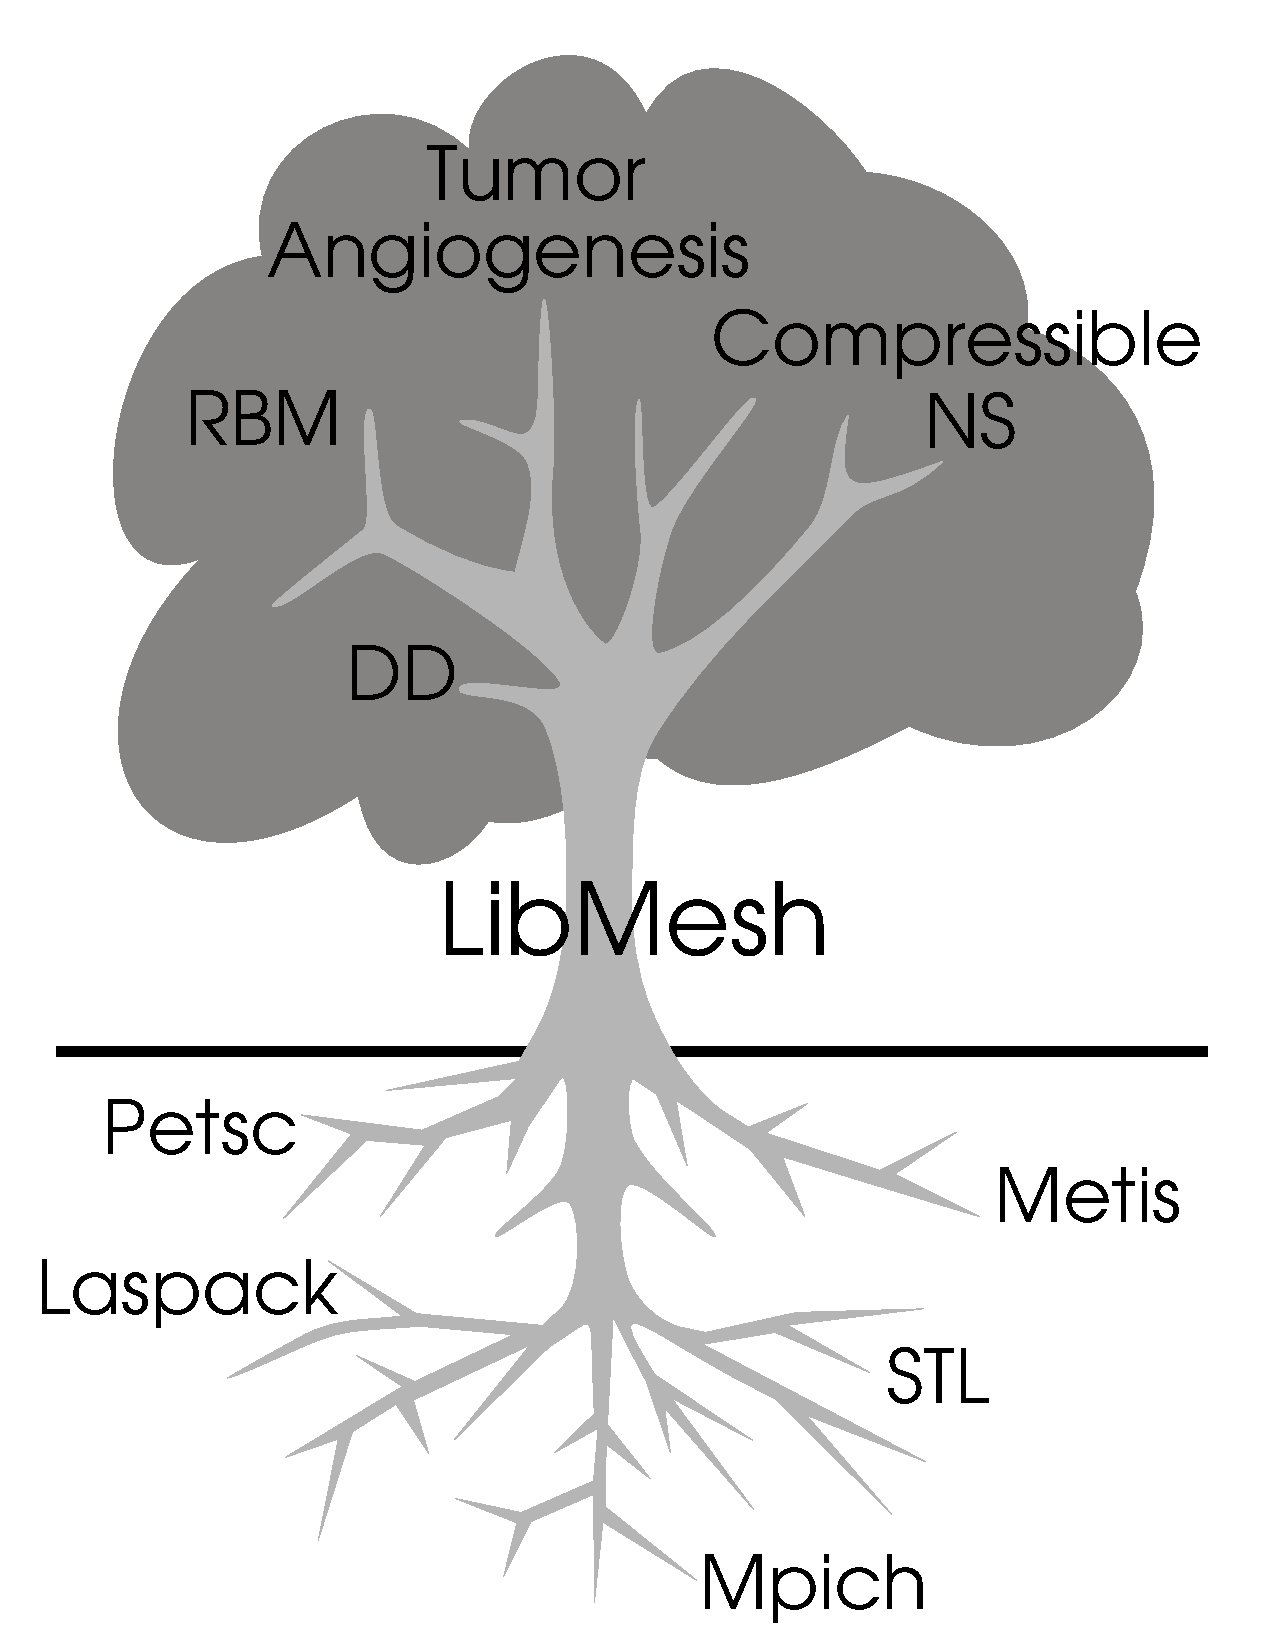
\includegraphics[width=.9\textwidth]{mytreeandroots_allnames}
    \end{center}
  \end{minipage}
  \begin{minipage}[h]{.35\textwidth}
    \begin{block}{Library Structure}
      \begin{itemize}
        %\small
    \item Basic libraries are \libMesh{}'s ``roots''
    \item Application ``branches'' built off the library ``trunk''
      \end{itemize}
    \end{block}
  \end{minipage}



\end{frame}
